\subsection{Simulation 4}
\label{sec:sim4}

% Esta seccion es varying sample size

The purpose of the final section in the simulation study is to observe how the methods behave when dealing with different population sample sizes $N$. Once again, the challenge here is that a high degree of conditional imbalance may lead to an additional dimensionality problem as the sample size gets smaller. To avoid this issue from affecting the analysis of the methods' performance, I will keep the number of regressors at a constant $k=10$ throughout the simulation. Although this means that the exercise is limited to scenarios where only the marginal imbalance varies, Simulation \ref{sec:sim3} has already covered cases with very small subsample sizes and high conditional imbalance that have shown the methods to perform poorly. Therefore, working with a smaller $k$ could shed light on how the methods perform on different sample sizes without the interference of dimensionality issues.\\

As all techniques primarily rely on asymptotics for consistency, particularly the LCC method, it is anticipated that the bias and variance will be inflated when $N$ and, consequently, $N_s$ decrease. However, the performance of the methods on small sample sizes is not solely determined by the size of the entire population but also relies on a combination of the sample size $N$ and the amount of marginal imbalance present in the sample. The sample sizes utilized in this analysis may not correspond to massive dataset setups because of computational limitations. However, they serve the purpose of providing a scaled-up understanding of the techniques' behavior as $N$ changes.\\

Let $N=\{10^5, 10^4, 5000, 2000, 1500 \}$ be the possible full population sizes to be used. As mentioned before, I will also be varying the marginal imbalance levels $P(Y=0)=\{0.7, 0.8, 0.9, 0.95\}$ for each of the sample sizes in order to get a more comprehensive analysis for distinct DGPs. Table \ref{tab:sim4-Ns} in the Appendix shows the summary statistics of LCC subsample sizes used to pick the fixed subsamples for this exercise, whereas Tables \ref{tab:sim4-0.7}, \ref{tab:sim4-0.8}, \ref{tab:sim4-0.9}, and \ref{tab:sim4-0.95} contain all the numerical results for all the simulations in a similar manner as the tables presented in Simulation \ref{sec:sim3}.\\

Figure \ref{fig:all_biases} displays a visual representation of the empirical squared bias outcomes for all simulation setups. Individually, the x-axis in each graph shows the squared root of the squared bias, and the y-axis displays the log transformation of the fixed subsample size $N_s$ used for each setup. As expected, the squared bias decreases as $N_s$ increases as a result of a larger population sample size. Panel A and B depict the simulation findings for a mild marginal imbalance of $P(Y=0)=0.7$ and $P(Y=0)=0.8$, respectively. In both cases, the LCC outperforms the other two subsampling methods in terms of squared bias for all $N_s$ values, even for very small subsample sizes. CC and WCC seem to perform quite similarly for the lowest level of imbalance, but, as expected, WCC starts to perform worse as the imbalance level increases. The most dramatic deterioration, however, is seen by LCC in scenarios with high to severe marginal imbalance and small sample sizes, as shown in Panels C and D. Specifically, the problem arises in cases with a full sample size of $1,500$ for $P(Y=0)=0.9$ and $2,000$ or lower for $P(Y=0)=0.95$. The explosion in the bias is so severe that it actually reaches $10^{25}$ for the last corner case.
\\

\begin{figure}[ht]
    \centering
    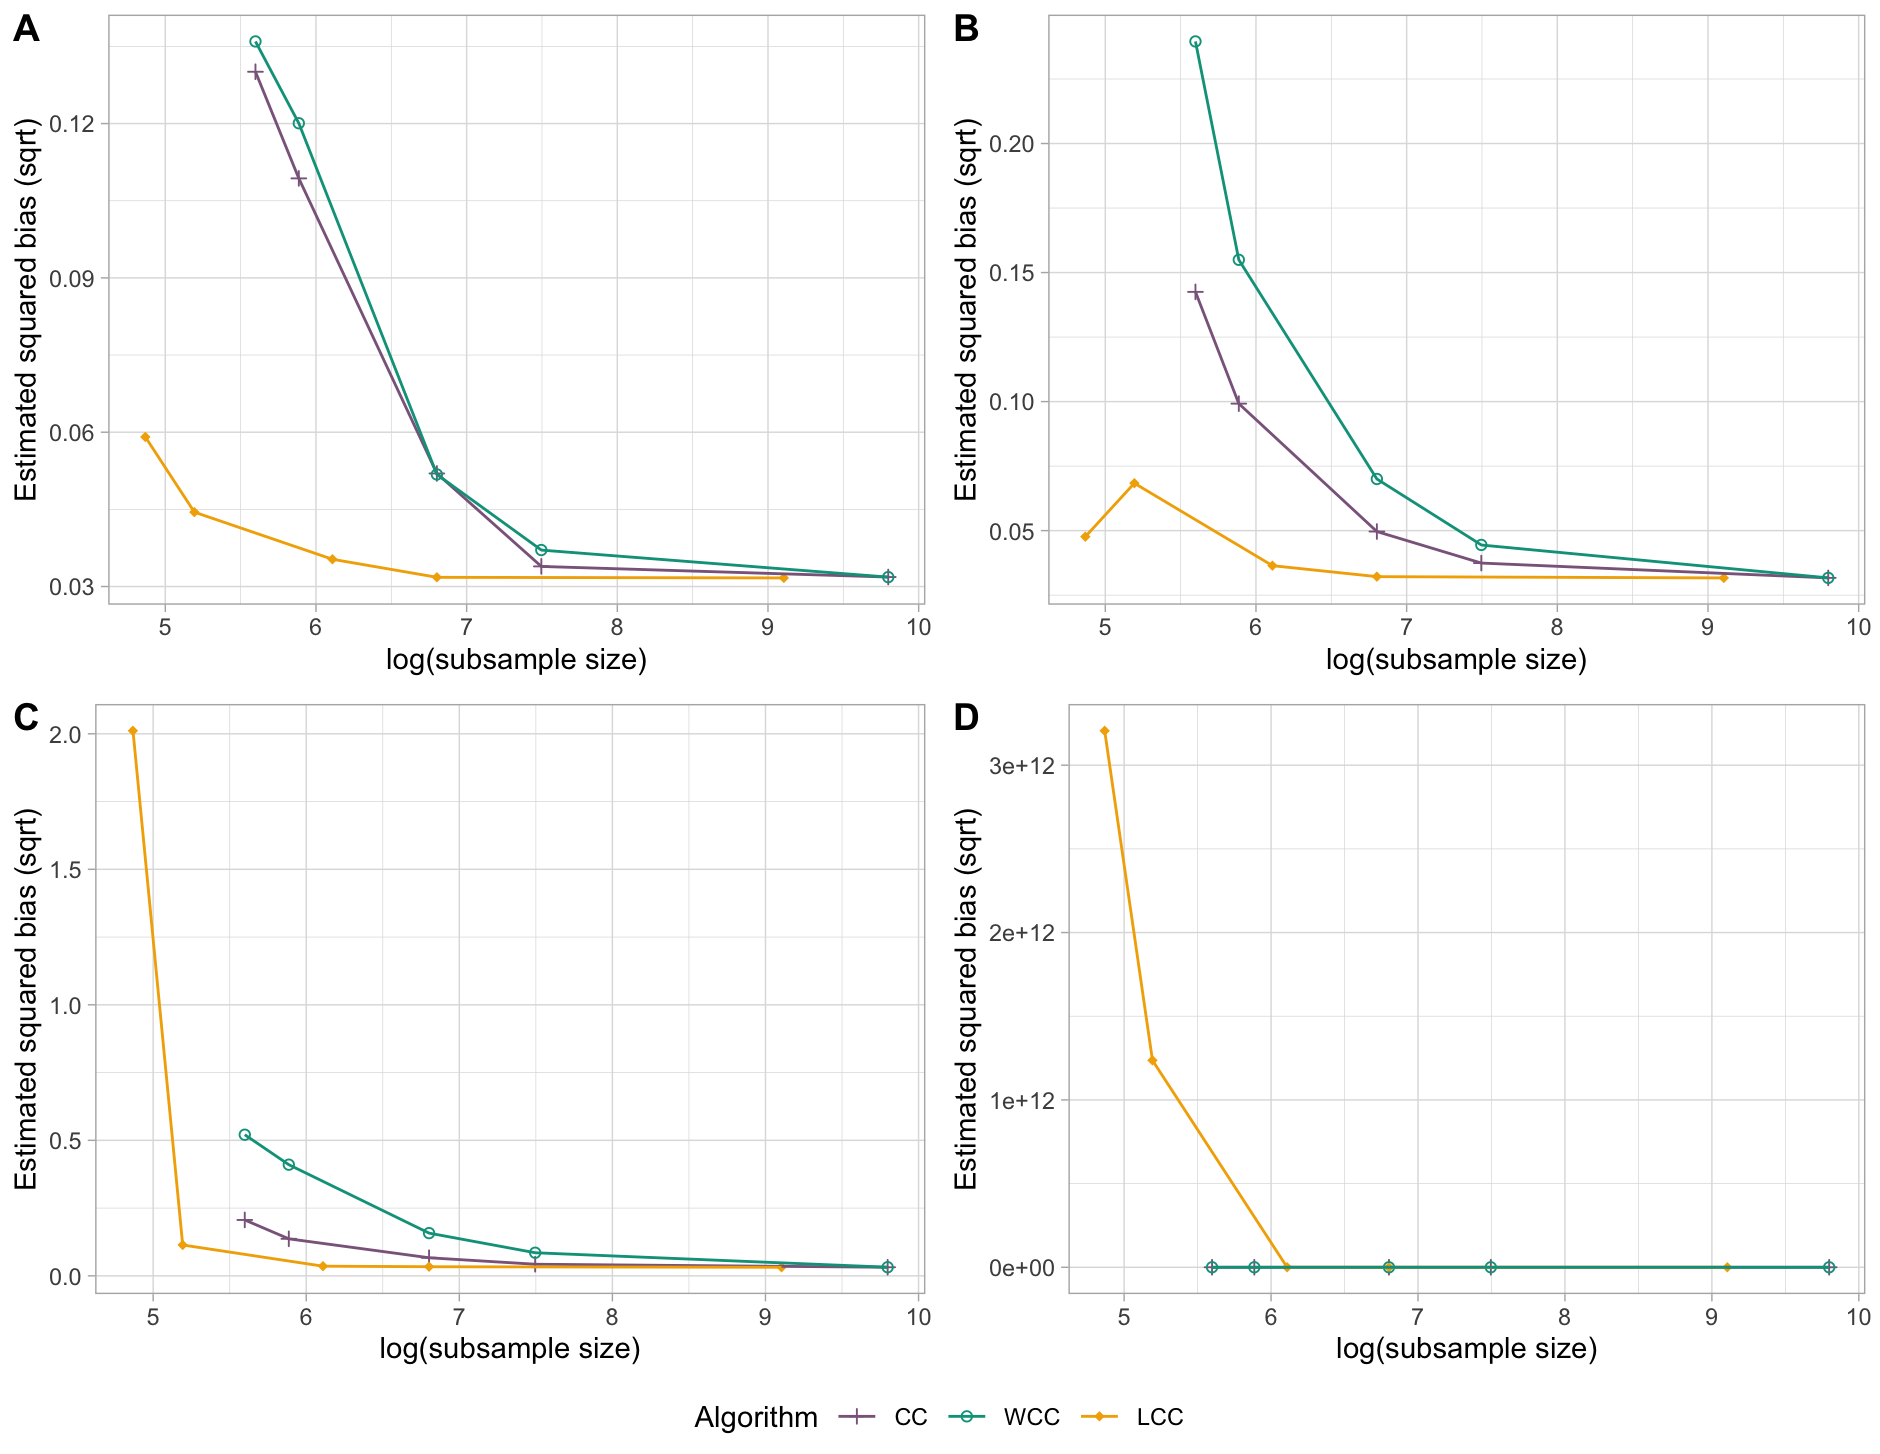
\includegraphics[width=\textwidth]{2_Figures/all_bias_smallk.png}
    \caption[Simulation 4 - Relationship between empirical squared bias and subsample size by method]{Simulation 4 - Relationship between estimated squared bias and subsample size by Algorithm under different levels of marginal imbalance.
    \textbf{Panel A:} Mild imbalance $P(Y=0)=0.7$.
    \textbf{Panel B:} Mild-high imbalance $P(Y=0)=0.8$.
    \textbf{Panel C:} High imbalance $P(Y=0)=0.9$.
    \textbf{Panel C:} Severe imbalance $P(Y=0)=0.95$.}
    \label{fig:all_biases}
\end{figure}

The performance of the methods in terms of variance is shown in Figure \ref{fig:all_vars}. Here, for mild levels of marginal imbalance illustrated in Panels A and B, the algorithms perform very similarly, with LCC doing as well as the other two. This similarity can be attributed to the fact that when there is low conditional imbalance, LCC does not have any significant advantage over the other two methods, resulting in a similar performance between the three. Once again, however, problems arise as $N$ gets smaller and $P(Y=0)$ becomes larger, as in the last two panels. As with the squared bias, the variance of LCC also gets extremely inflated for sample sizes of $2,000$ or lower and large to severe marginal imbalance. \\

\begin{figure}[ht]
    \centering
    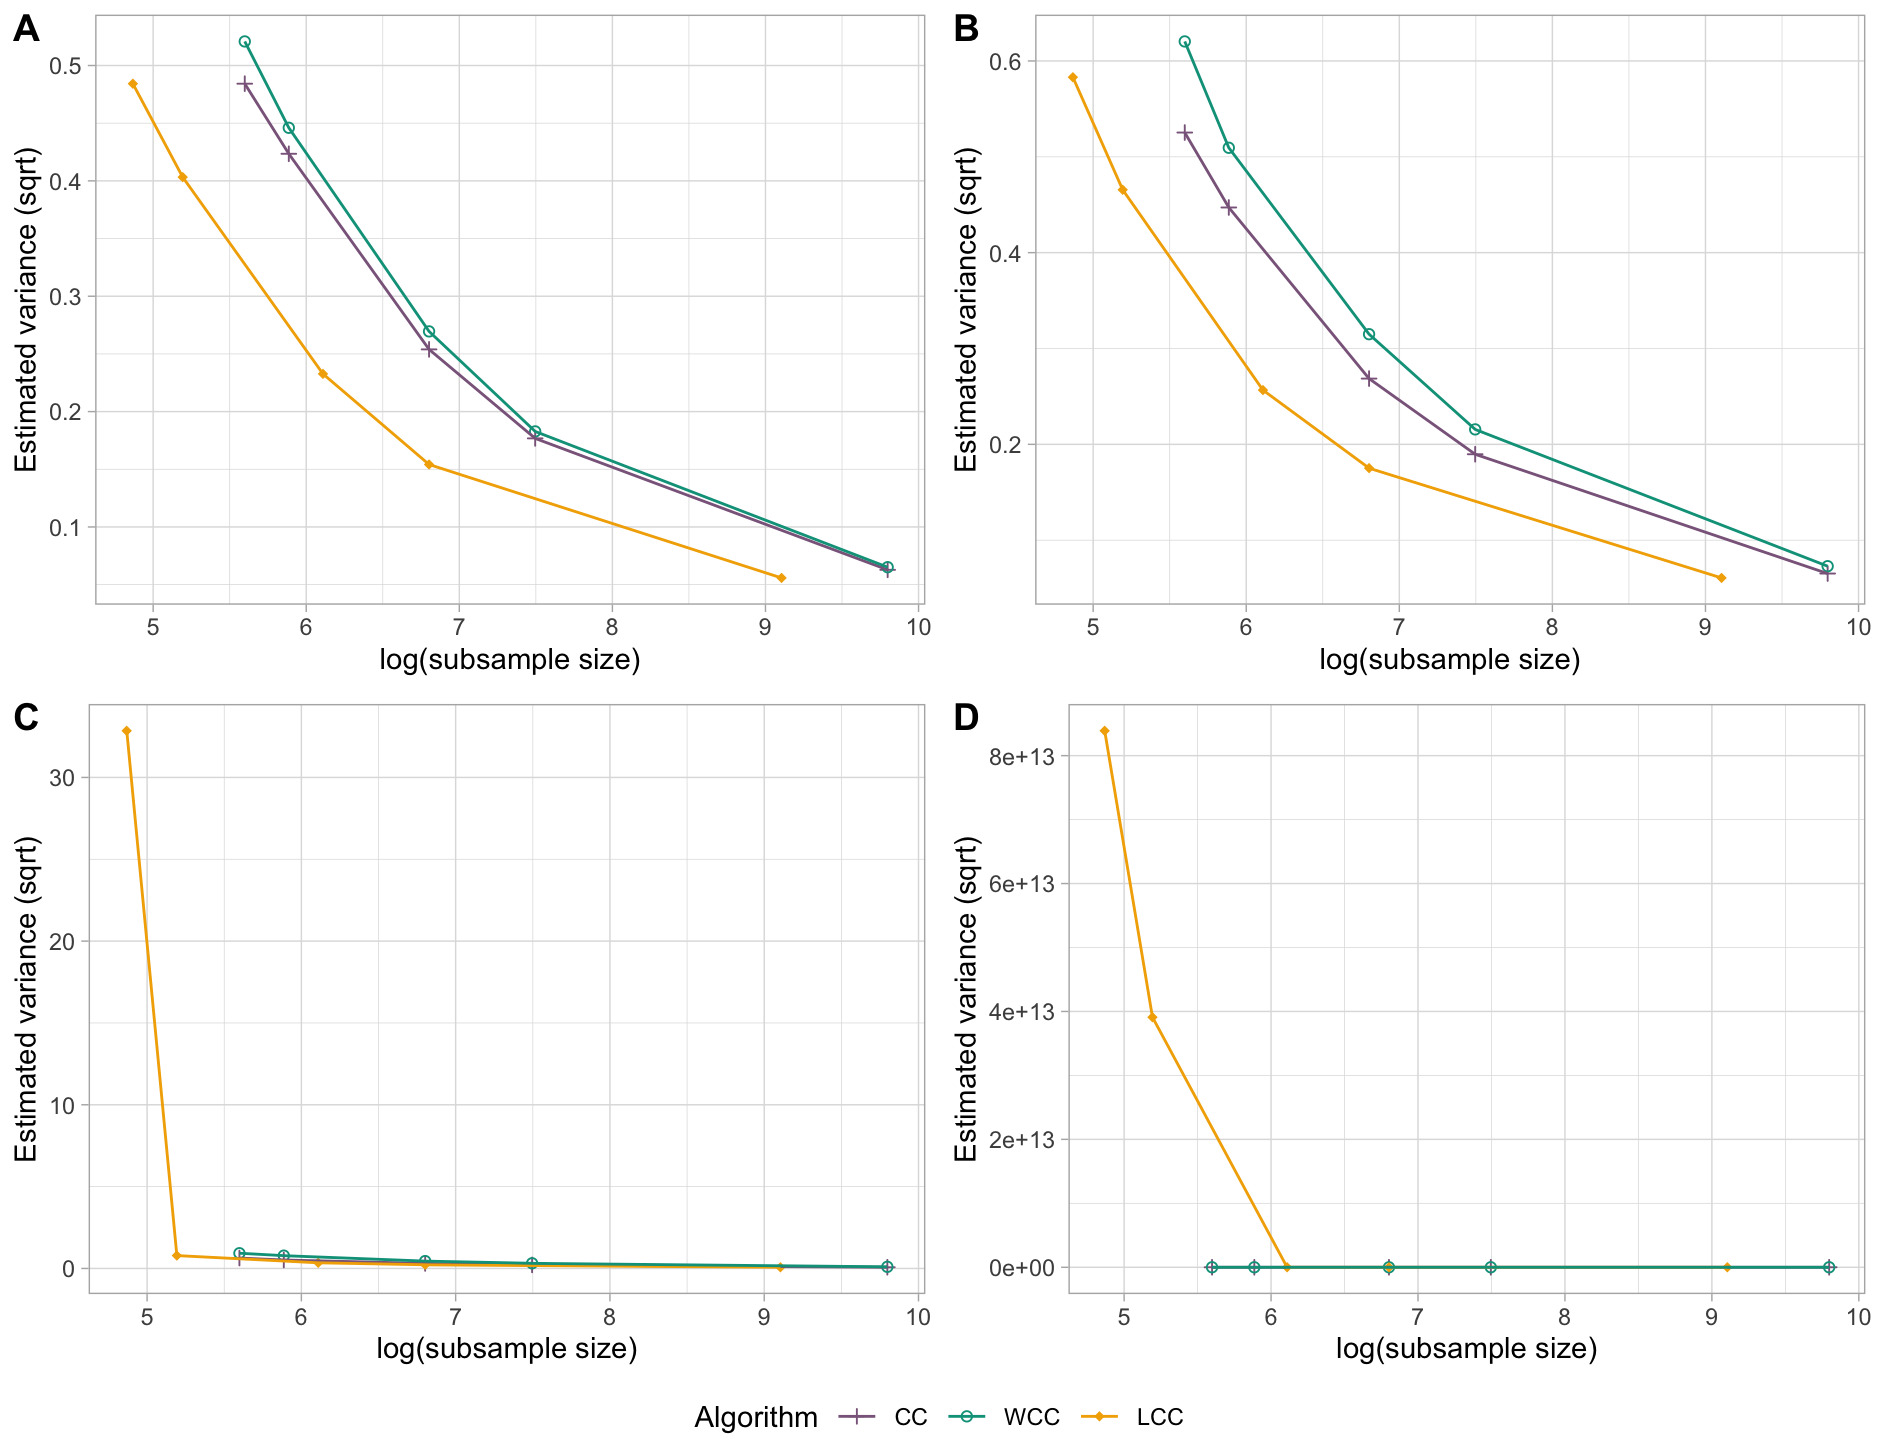
\includegraphics[width=\textwidth]{2_Figures/all_var_smallk.png}
    \caption[Simulation 4 - Relationship between empirical variance and subsample size by method]{Simulation 4 - Relationship between estimated variance and subsample size by Algorithm under different levels of marginal imbalance.
    \textbf{Panel A:} Mild imbalance $P(Y=0)=0.7$.
    \textbf{Panel B:} Mild-high imbalance $P(Y=0)=0.8$.
    \textbf{Panel C:} High imbalance $P(Y=0)=0.9$.
    \textbf{Panel C:} Severe imbalance $P(Y=0)=0.95$.}
    \label{fig:all_vars}
\end{figure}

Thus, a reasonable conclusion is that in ``corner-case" scenarios, LCC will usually be the worst method among the three. Looking at Table \ref{tab:sim4-0.95}, a more appropriate choice among the subsampling methods will be the CC algorithm since WCC also shows poor performance due to the variance induced from the disproportional weights in high imbalance setups. CC not only seems pretty stable in these scenarios, but it is the one method that gets closer to the bias and variance empirical benchmark of logistic regression. Once again, it is important to note that under such a small $N$, the logistic regression will always be preferred as it is still the method that shows the lowest squared bias and variance, and it is still a case under which it would be feasible to compute the full sample $\hat{\theta}_{MLE}$. This exercise serves as a demonstration, however, that LCC could fail in instances where the imbalance is extremely severe, even for large $N$. \\

\textcite{wang2018optimal} exhibit similar conclusions. The authors conducted simulation experiments and showcased the performance of various two-step subsampling techniques in terms of empirical MSE under different subsample size ratios. LCC was used as a comparison estimator together with uniform subsampling. Their findings indicate that LCC does not perform well on small subsample sizes, mainly because the effective sample size is smaller than the other methods under study. They conclude that LCC fails to approximate the full sample parameters under such conditions.


















% **TODO**: Here, I need to explain that this comes from a given population size and that the subsample sizes are actually determined by LCC (CC AND WCC are just twice as the subsample size of LCC, following \cite{hastie2014}) and the $N_s$ of LCC is dictated by k, and N (population size). IMPORTANT: compare the graphs to .

    






